\section{Аналіз рішення}
 Анализ, согласно критериям как работает, пути улучшения (таблица сравнения с существующими подходами, графики, диаграммы)

\subsection{Порівняльний аналіз}
Було проведено порівняльний аналіз рішення з існуючими реалізаціями для підтердження ефективності використання даного алгоритму. Обрані такі критерії для побудови порівняльної таблиці:

\begin{itemize}
	\item відхилення від еталонної величини;
	\item середнє квадратичне відхилення
	\item Підтверджено значно більші показники швидкодії моделі, розробленої за допомогою даного підходу.
\end{itemize}


Також для найкращої моделі та гібридної моделей були побудовані таблиці помилок (\textit{confusion matrix}) - матриці, що допомагають візуалізувати ефективність алгоритмів. Кожна колонка містить кількість результатів в передбачуваному класі, в той час як кожен рядок містить дійсну кількість елементів у класі (рис. \ref{fig:confusion_matrix}).

\begin{figure}[h!]
  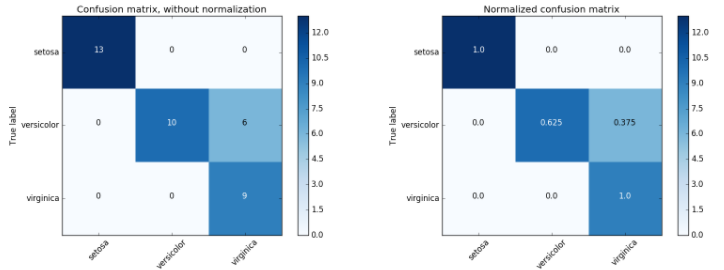
\includegraphics[width=\linewidth]{figures/confusion_matrix.png}
  \caption{Приклад матриці помилок для вхідного набору даних Iris}
  \label{fig:confusion_matrix}
\end{figure}

Результати для моделі \textit{Support Vector Machines} та побудованої гідбридної моделі (табл. \ref{tab:confusion_matrix}) дають змогу зрозуміти, обидві моделі відносять елементи до однакових класів. Це означає, що хоч і точніть передбачення не є максимально можливою, проте дозволяє показати стабільні консистенті результати для обох моделей, а це, у свою чергу, дозволяє підтверджувати надійність розроблюваного підходу.

\begin{table}[h!]
	\begin{tabularx}{\textwidth}{|X|X|X|X|}
    \hline
     & setosa & versicolor & virginica \\ \hline
    setosa & 7 & 0 & 0 \\ \hline
    versicolor & 0 & 10 & 2 \\ \hline
    virginica & 0 & 0 & 11 \\
    \hline
    \end{tabularx}
\caption{Матриця помилок} \label{tab:confusion_matrix}
\end{table}

Швидкодія роботи на різних вхідних даних
 \subsection{Отримані результати та шляхи покращення}
 Отже, в результаті отримана реалізація показала відповідність усім висунутим вимогам та продемонструвала стабільні показники незалежно від виду та об'єму вхідних даних. На поточному етапі такі результати повністю задоволняють як користувачів алгоритму, так і розробників, які бажають покращити алгоритм чи модифікувати його будь-яким чином для забезпечення кращих показників точності чи швидкодії.

Серед напрямків для покращення алгоритму можна виділити такі основні:

\begin{itemize}
	\item Визначення оптимального алгоритму не шляхом повного перебору існуючих моделей, а за допомогою деякої евристики. Зараз для вхідних даних необхідно побудувати всі моделі, користуючись медотом повного перебору () і виконати їхнє порівняння за деякою обраною метрикою. Лише після цього на основі кращої моделі буде побудована наша гібридна модель. Якщо ж скористатися деяким набором правил, евристикою чи іншими додатковими знаннями в доменній залузі - можна обмежити кількість моделей, що будуть побудовані, таким чином в декілька разів зменшити витрати на час на етапі побудови моделей. Виграш буде значно відчутний на великій кількості моделей за умови, що лише кілька з них дійсно показують стабільно найкращі результати для схожих вхідних даних. Однією із можливих реалізацій такого прийому може бути додаткова модель-класифікатор, що буде на основі вхідних даних обирати клас алгоритмів (деяке значення Т), для яких варто проводити побудову моделей. Іншим варіантом може бути підтримка структури у вигляді словника, що буде зберігати наперед визначені користувачем набори типу "критерій"-"клас алгоритмів" і значно швидше (за лінійний час) буде обирати потрібну множину алгоритмів. Останній підхід є значно швидшим, але вимагає додаткової початкової ініціалізації та втручання людини для підготовки такого словника.
	\item Запуск побудови кожної моделі в окремому потоці. Процес побудови моделі є процесом, що в першу чергу вимагає процесорний час для виконання (\textit{cpu-bound}), тому з апаратної точки зору прискорити його роботу можливо за рахунок розпаралелювання на декількох ядрах процесора. Найпростішим варіантом є використання багатоядерних процесорів і виконнання алгоритму на окремому ядрі. Сучасні відеокарти з підтримкою технологій \textit{Nvidia CUDA} та \textit{AMD OpenCL} теж можуть бути використані для запуску даних алгоритмів. Порівняння показують, що використання відеокарт для схожих обрахунків може надати приріст у розмірі 90-95х кратного прискорення роботи. Аналогічним чином можна скористатися розподіленими та багатопроцесрними системами, коли алгоритми будуть виконуватися окреми на різних машинах в межах одного кластеру. Головним недоліком таких систем є підвищення порогу входження для розробки, адже це вимагає додаткових знань як для написання коду (\textit{C++, MPI, OpenMPI}), так і розуміння архітектури розподілених систем вцілому. Наприклад, для написання алгоритму для кластеру потрібно розуміти, що кожна модель на окремій ноді кластеру повинна мати доступ до вхідного датасету, а отже потрібно забезпечити централізований неблокуючий доступ до даних або реалізувати можливість спільної пам'яті (\textit{shared memory}), що теж вимагає додаткових зусиль з точки зору програміста. З переваг варто відмітити однократність даної операції та практично необмежений лінійний ріст ефективності пропорційно до кількості початкових алгоритмів.
	\item Під час сумісної роботи над проектом виникає необхідність обміну даними між розробниками. Науковці хочуть мати змогу надсилати моделі іншим, а також мати змогу їх зберегти для подальшого використання. Тому ще одним можливим шляхом для вдосконалення може бути можливість серіалізації моделей. Таким чином модель можна буде побудувати і зберегти в бінарному форматі на одному комп'ютері, а потім використати в майбутньому без необхідності повторної її перебудови. Звісно такий підхід працює лише для одного набору вхідних даних, тому область його застосування досить обмежена. Проте, якщо над деякими даними працює команда науковців, саме це дасть змогу швидко обмінюватися результатами чи використовувати напрацювання інших. Найпростішою реалізаціює тут може бути знімок об'єкта у пам'яті, але таким чином втрачається кросплатформенність та машинонезалежність. Вбудовані підходи до серіалізації (наприклад, \textit{pickle}) також будуть страждати від подібних нюансів. Саме тому необхідно буде розробити додатковий алгоритм для серіалізації моделей, що і є головним фактором, який стримує додавання даної можливості до існуючого коду.
\end{itemize}

Розглянуті напрямки покращення дозволять збільшити швидкодію програми вцілому, а також спростити використання її в межах команди науковців, а тому доцільно розглянути подальшу роботу над проектом саме в одному із запропонованих напрямків.